\documentclass[caption=numbered]{beamer}
\usetheme[color=screen]{UniBern}

%\setbeameroption{show notes}
\includeonlyframes{current}

\usepackage{lmodern}
\usepackage[english]{babel}
\usepackage{microtype}
\usepackage{textcomp}
\usepackage[backend=biber, style=alphabetic, url=false]{biblatex}
\addbibresource{../../Documents/library.bib}
\usepackage{graphicx}
\usepackage{caption}
	\captionsetup[figure]{labelformat=empty} % No 'figure' in figures
\usepackage{tikz}
	\usetikzlibrary{spy}
\usepackage[detect-all=true, range-phrase=--, range-units=single]{siunitx}
\usepackage{csquotes}
\usepackage{animate}
\usepackage{sparklines}
\usepackage{booktabs}
\usepackage[absolute,overlay]{textpos} %for the \source{} command
\usepackage{gitinfo2}
\usepackage{xspace}
\usepackage{todonotes}
	\presetkeys{todonotes}{inline}{} % http://tex.stackexchange.com/a/12331/828
\usepackage{hyperref}

\hypersetup{pdfstartview={Fit}}
\setbeamertemplate{caption}{\insertcaption}
\setbeamertemplate{caption}[numbered]

\newcommand{\imsize}{\linewidth}
\newlength\imagewidth % needed for scalebars
\newlength\imagescale % ditto
\newcommand{\uct}{\si{\micro}CT\xspace}
\newcommand{\uaf}{\si{\micro}AngioFil\xspace}

\newcommand{\source}[1]{%http://tex.stackexchange.com/a/48485/828
	\begin{textblock*}{4cm}(8.7cm,8.6cm)%
		\begin{beamercolorbox}[ht=0.5cm,right]{framesource}%
			\tiny\usebeamerfont{framesource}\usebeamercolor[fg]{framesource} Source: {#1}%
		\end{beamercolorbox}%
	\end{textblock*}%
}

% Biblatex: http://tex.stackexchange.com/a/13076/828
% % Format bibliography for beamer
% % http://tex.stackexchange.com/a/10686/828
% \renewbibmacro{in:}{}
% % http://tex.stackexchange.com/a/13076/828
% \AtEveryBibitem{\clearfield{title}}
% \AtEveryBibitem{\clearfield{journaltitle}}
% \AtEveryBibitem{\clearfield{year}}
% \AtEveryBibitem{\clearfield{pages}}
% \AtEveryBibitem{\clearfield{volume}}
% \AtEveryBibitem{\clearfield{number}}
% %http://tex.stackexchange.com/a/40710/828
% \usepackage{xpatch}
% \xpatchbibmacro{month}{%
%   \printtext[parens]%
% }{%
%   \setunit*{\addperiod\space}%
%   \printtext%
% }{}{} 

\subtitle{Several examples as well as details in lung and brain imaging}
\author[David Haberthür]{David Haberthür \and\tiny Adolfo Odriozola \and Ruslan Hlushchuk \and Valentin Djonov}
\institute{Institute of Anatomy\\Universität Bern}
\date{February 9, 2017\\Internal seminar@Institute of Anatomy}

%\useoutertheme{split}

\begin{document}
\title[\si{\micro}CT in biological studies]{\si{\micro}CT-imaging at the Institute of Anatomy} % http://tex.stackexchange.com/a/144445/828

\defbeamertemplate{footline}{unibe}
{%
	\usebeamercolor[fg]{page number in head/foot}%
	\usebeamerfont{page number in head/foot}%
	\hspace*{\fill}%
	\insertshortauthor%
	\hspace*{\fill}%|\hspace*{\fill}%
	\insertshorttitle%
	\hspace*{\fill}%|\hspace*{\fill}%
	v.~\gitAbbrevHash%
	\hspace*{\fill}%|\hspace*{\fill}%
	\insertframenumber\,/\,\insertpresentationendpage%
	\hspace*{\fill}%
	\vskip2pt%
}
\setbeamertemplate{footline}[unibe]

{
\setbeamertemplate{footline}{} % http://tex.stackexchange.com/a/18829/828
\begin{frame}
  \titlepage
\end{frame}
}
\addtocounter{framenumber}{1}

\begin{frame}{Contents}
	\tableofcontents
\end{frame}

\section{Theory}
\renewcommand{\imsize}{0.95\textheight}
\begin{frame}{Theory computed tomography}
	\begin{columns}
		\begin{column}{0.7\linewidth}
			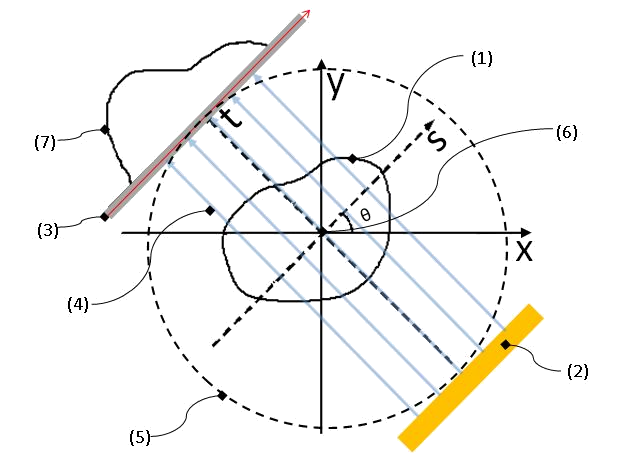
\includegraphics[width=\imsize]{img/CT_PRINCI_PB}
				\source{\href{https://commons.wikimedia.org/wiki/File:CT_PRINCI_PB.jpg}{enwp.org/tomography}}	
		\end{column}
		\begin{column}{0.4\linewidth}
			\begin{enumerate}
				\item Object
				\item Parallel light source
				\item Screen
				\item Transmitted beam
				\item Datum circle
				\item Origin
				\item 1D image
			\end{enumerate}
		\end{column}
	\end{columns}
\end{frame}

\section{Current and ongoing projects}
\begin{frame}{Zebrafish}
	\renewcommand{\imsize}{\linewidth}%
	\begin{figure}%
		\pgfmathsetlength{\imagewidth}{\imsize}%
		\pgfmathsetlength{\imagescale}{\imagewidth/1651}%
		\def\x{1020}% scalebar-x starting at golden ratio of image width of 1651px = 1020
		\def\y{391}% scalebar-y at 90% of image height of 434px = 391
		\begin{tikzpicture}[x=\imagescale,y=-\imagescale]%
			\node[anchor=north west, inner sep=0pt, outer sep=0pt] at (0,0) {\includegraphics[width=\imagewidth]{img/{{zebrafish_rec_voi_side}}}};
			% 1615px = 35.48 > 100px = 2198um > 23px = 500um, 5px = 100um
			%\draw[|-|,blue,thick] (20,154) -- (1634,127) node [sloped,midway,above,fill=white,semitransparent,text opacity=1] {\SI{35.487480000000005}{\milli\meter} (1615px) TEMPORARY!};
			\draw[|-|] (\x,\y) -- (\x+234.19,\y) node [midway,above] {\SI{5}{\milli\meter}};
		\end{tikzpicture}%
		\caption{Visualization of a tomographic scan of a zebrafish, fixed in \SI{4}{\percent} PFA.}%
	\end{figure}%
\end{frame}

\begin{frame}{Rat head}
	\renewcommand{\imsize}{0.9\linewidth}%
	\begin{figure}%
		\pgfmathsetlength{\imagewidth}{\imsize}%
		\pgfmathsetlength{\imagescale}{\imagewidth/1400}%
		\def\x{865}% scalebar-x starting at golden ratio of image width of 1400px = 865
		\def\y{560}% scalebar-y at 90% of image height of 622px = 560
		\begin{tikzpicture}[x=\imagescale,y=-\imagescale]
			\node[anchor=north west, inner sep=0pt, outer sep=0pt] at (0,0) {\includegraphics[width=\imagewidth]{./img/{{ratwholehead_rec_side}}}};
			%\spy [red] on (1100,322) in node at (0,0) [anchor=north west];
			% 1358px = 47.76mm > 100px = 3517um > 14px = 500um, 3px = 100um
			%\draw[|-|,blue,thick] (23,291) -- (1380,311) node [sloped,midway,above,fill=white,semitransparent,text opacity=1] {\SI{47.76}{\milli\meter} (1358px) TEMPORARY!};
			\draw[|-|] (\x,\y) -- (\x+140,\y) node [midway,above] {\SI{5}{\milli\meter}};
		\end{tikzpicture}%
		\caption{Visualization of a tomographic scan of a rat head, instilled with \uaf and fixed in \SI{4}{\percent} PFA.}%
	\end{figure}%
\end{frame}

\begin{frame}{Rat brain vessels}
	\renewcommand{\imsize}{\linewidth}%
	\begin{columns}
		\begin{column}{0.618\linewidth}
			\pgfmathsetlength{\imagewidth}{\imsize}%
			\pgfmathsetlength{\imagescale}{\imagewidth/1950}%
			\def\x{1205}% scalebar-x starting at golden ratio of image width of 1950px = 1205
			\def\y{1230}% scalebar-y at 90% of image height of 1367px = 1230
			\begin{tikzpicture}[x=\imagescale,y=-\imagescale]
				\node[anchor=north west, inner sep=0pt, outer sep=0pt] at (0,0) {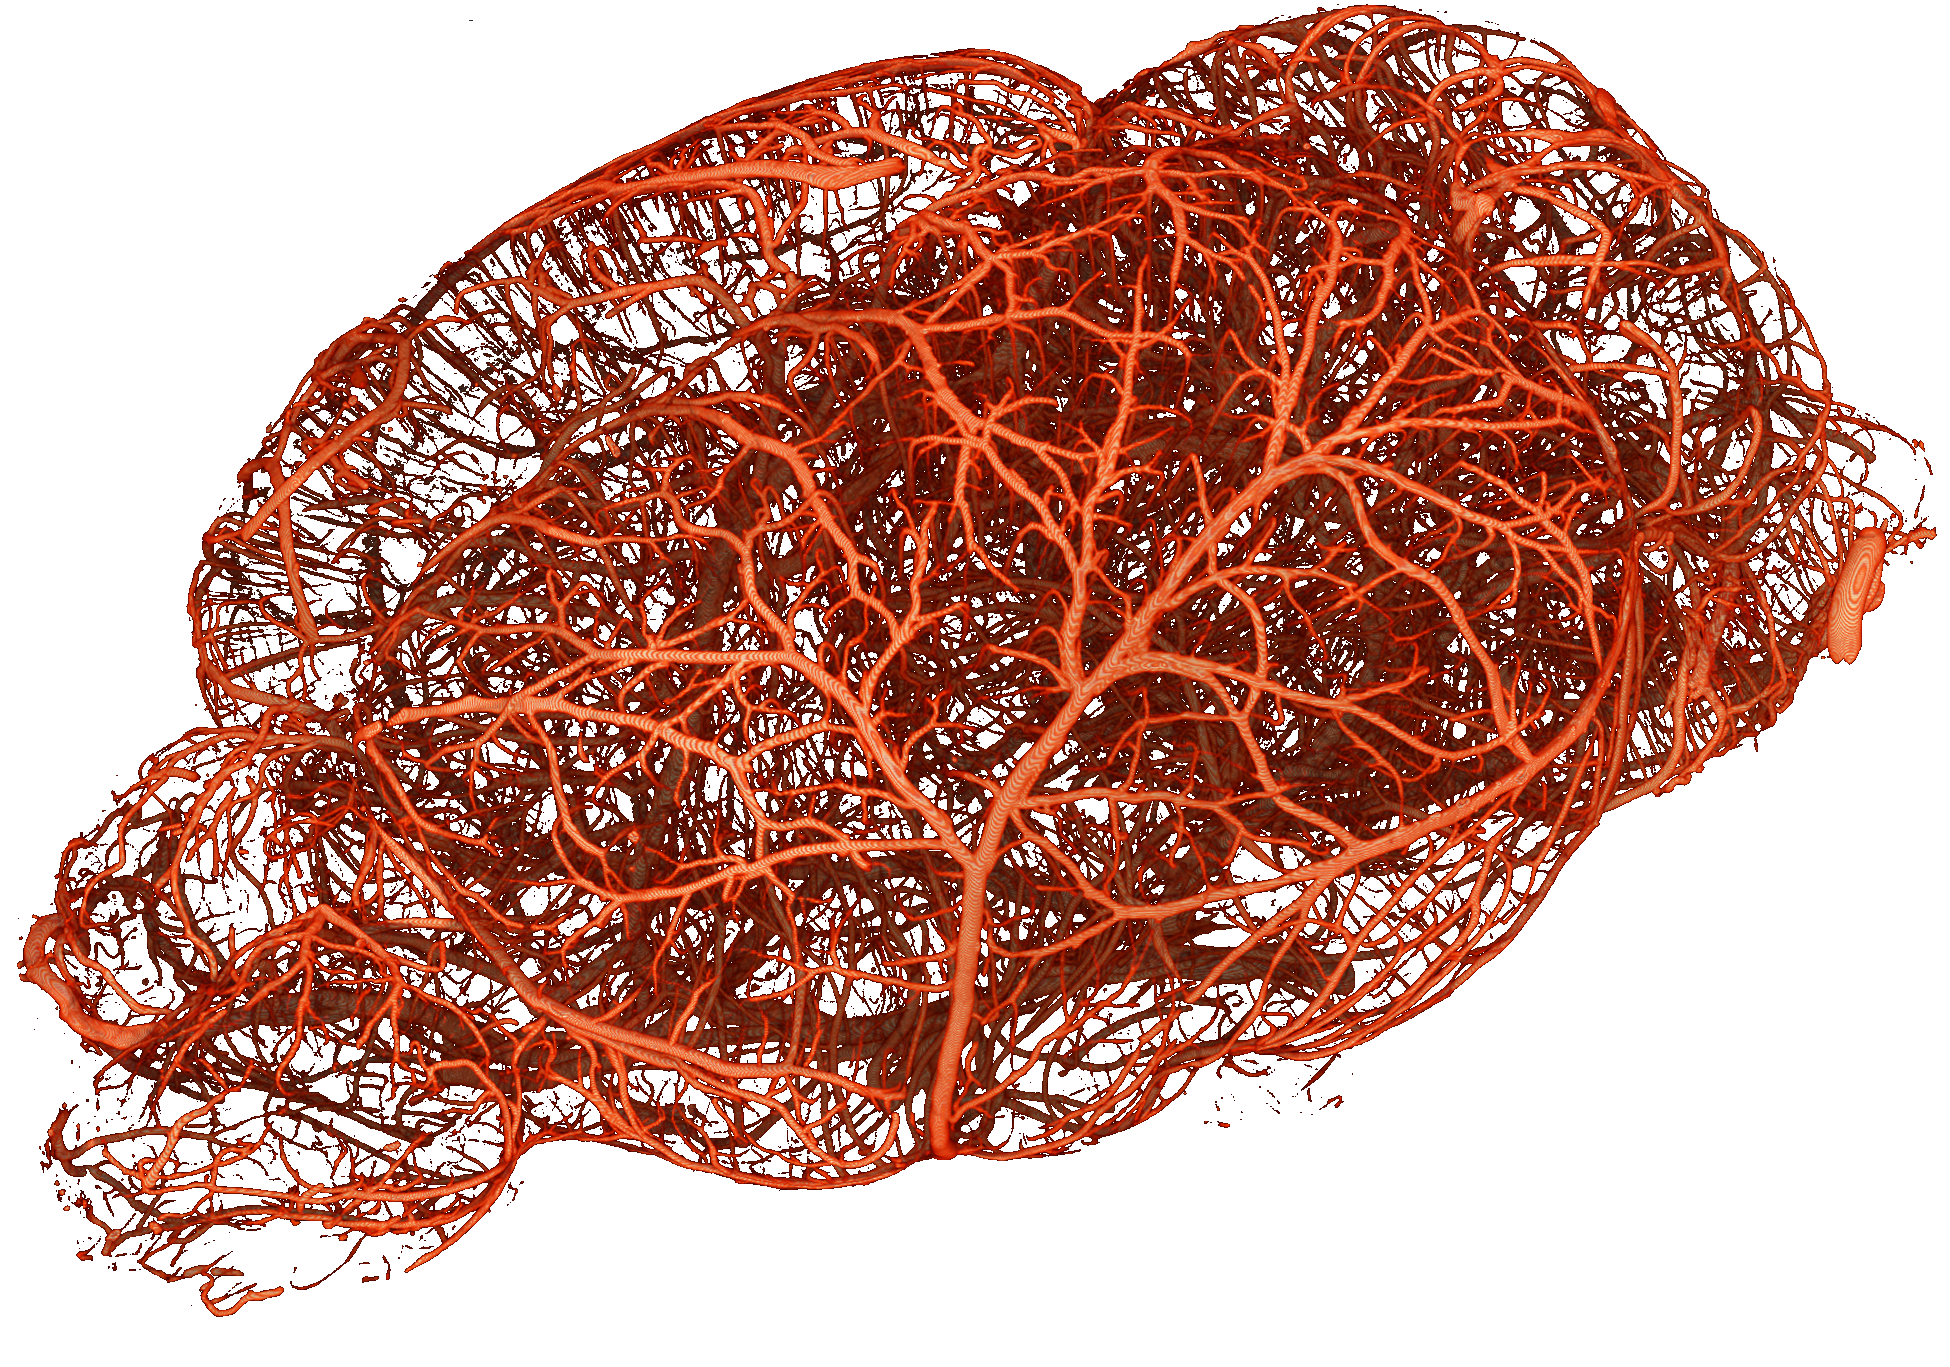
\includegraphics[width=\imagewidth]{img/Ebene_25}};
				% 1949px = 20.0mm > 100px = 1026um > 49px = 500um, 10px = 100um
				%\draw[|-|,blue,thick] (39,1222) -- (1722,239) node [sloped,midway,above,fill=white,semitransparent,text opacity=1] {\SI{20.0}{\milli\meter} (1949px) TEMPORARY!};
				\draw[|-| ] (\x,\y) -- (\x+490,\y) node [midway,above] {\SI{5}{\milli\meter}};
				\node [anchor=center] (cb) at (2000,0) {Cerebellum};
				\draw [thick] (cb.west) to [out=-180, in=0] (1482,144);
				\node [anchor=center] (bs) at (2250,1500) {Brain stem};
				\draw [thick] (bs.west) to [out=180, in=-45] (1705,725);
				\node [anchor=center, text width=2cm, align=center] (ob) at (550,1500) {Olfactory bulbs};
				\draw [thick] (ob.west) to [out=180, in=180] (210,880);
				\draw [thick] (ob.west) to [out=180, in=180] (298,1116);
			\end{tikzpicture}
		\end{column}		
		\begin{column}{0.382\linewidth}
			Visualization of a tomographic scan of a \uaf-filled mouse brain.
		\end{column}
	\end{columns}
\end{frame}

\section{Assessing tumor/metastasis load in lungs}
\begin{frame}
	\frametitle{Tumor metastasis}
	\begin{itemize}
		\item Assessing tumor load in lungs
		\item KP-TNIK mice
		\item Stereology
	\end{itemize}
\end{frame}

\renewcommand{\imsize}{0.33\linewidth}
\begin{frame}
	\frametitle{Tumor load in lungs, KP-TNIK mice}
	\begin{columns}
		\begin{column}{0.8\linewidth}
			\pgfmathsetlength{\imagewidth}{\imsize}%
			\pgfmathsetlength{\imagescale}{\imagewidth/800}%
			\def\x{494}% scalebar-x starting at golden ratio of image width of 800px = 494
			\def\y{720}% scalebar-y at 90% of image height of 800px = 720
			\begin{tikzpicture}[x=\imagescale,y=-\imagescale]
			\node[anchor=north west, inner sep=0pt, outer sep=0pt] at (0,0) {\includegraphics[width=\imagewidth]{../../Documents/Collaborations/DKF_Lung/Overview/{{MAX_--11}}}};
			% 800px = 16.0mm > 100px = 2000um > 25px = 500um, 5px = 100um
			%\draw[|-|,blue,thick] (0,400) -- (800,400) node [sloped,midway,above,fill=white,semitransparent,text opacity=1] {\SI{16.0}{\milli\meter} (800px) TEMPORARY!};
			\draw[|-|] (\x,\y) -- (\x+250,\y) node [midway,above] {\SI{5}{\milli\meter}};
			\end{tikzpicture}%
			\begin{tikzpicture}[x=\imagescale,y=-\imagescale]
			\node[anchor=north west, inner sep=0pt, outer sep=0pt] at (0,0) {\includegraphics[width=\imagewidth]{../../Documents/Collaborations/DKF_Lung/Overview/{{MAX_--12}}}};
			\draw[|-|] (\x,\y) -- (\x+250,\y) node [midway,above] {\SI{5}{\milli\meter}};
			\end{tikzpicture}%
			\begin{tikzpicture}[x=\imagescale,y=-\imagescale]
			\node[anchor=north west, inner sep=0pt, outer sep=0pt] at (0,0) {\includegraphics[width=\imagewidth]{../../Documents/Collaborations/DKF_Lung/Overview/{{MAX_--13}}}};
			\draw[|-|] (\x,\y) -- (\x+250,\y) node [midway,above] {\SI{5}{\milli\meter}};
			\end{tikzpicture}%
			\\%
			\begin{tikzpicture}[x=\imagescale,y=-\imagescale]
			\node[anchor=north west, inner sep=0pt, outer sep=0pt] at (0,0) {\includegraphics[width=\imagewidth]{../../Documents/Collaborations/DKF_Lung/Overview/{{MAX_wt11}}}};
			\draw[|-|] (\x,\y) -- (\x+250,\y) node [midway,above] {\SI{5}{\milli\meter}};
			\end{tikzpicture}%
			\begin{tikzpicture}[x=\imagescale,y=-\imagescale]
			\node[anchor=north west, inner sep=0pt, outer sep=0pt] at (0,0) {\includegraphics[width=\imagewidth]{../../Documents/Collaborations/DKF_Lung/Overview/{{MAX_wt12}}}};
			\draw[|-|] (\x,\y) -- (\x+250,\y) node [midway,above] {\SI{5}{\milli\meter}};
			\end{tikzpicture}%
			\begin{tikzpicture}[x=\imagescale,y=-\imagescale]
			\node[anchor=north west, inner sep=0pt, outer sep=0pt] at (0,0) {\includegraphics[width=\imagewidth]{../../Documents/Collaborations/DKF_Lung/Overview/{{MAX_wt13}}}};
			\draw[|-|] (\x,\y) -- (\x+250,\y) node [midway,above] {\SI{5}{\milli\meter}};
			\end{tikzpicture}%
		\end{column}
		\begin{column}{0.15\textwidth}
			\begin{itemize}
				\item KO
				\item WT
			\end{itemize}
		\end{column}
	\end{columns}
\end{frame}

\begin{frame}{Tumor load in lungs, KP-TNIK mice. Top: KO, bottom: WT}
	\renewcommand{\imsize}{0.85\linewidth}  
	\animategraphics[palindrome,width=\imsize]{12}{../../Documents/Collaborations/DKF_Lung/movieframes/out-}{001}{255}
\end{frame}

\section{Lung fibrosis}
\begin{frame}{Backstory}
	\begin{itemize}
		\item Lung fibrosis grading \cite{Ashcroft1988a}
		\item \emph{Correct} sampling for proper assessment
		\item \uct is a tool to help grade fibrosis
		\begin{itemize}
			\item Detect and grade fibrosis
			\item Get indications where to perform the sampling
		\end{itemize}
		\item Cancer metastasis (\SI{2}{year} after radiation treatment fibrosis is induced)
		\item Cancer treatment
		\begin{itemize}
			\item Antiangiogenesis (failed)
			\item Radiation therapy, namely MRT \cite{Bronnimann2016} (probably better citation needed)!
		\end{itemize}
	\end{itemize}
\end{frame}

\begin{frame}
	\renewcommand{\imsize}{0.25\linewidth}  
	\frametitle{Multimodal imaging: \uct and 3View, correlated imaging}
	\begin{itemize}
		\item Problem: Fibrose grading \cite{Hubner2008} and sampling location
		\item<2> \uct
		\item<2> serial block-face scanning electron microscopy (\href{http://www.gatan.com/products/sem-imaging-spectroscopy/3view-system}{3View})
		\item<2> Registration of datasets, from overview to ultrafine structure
		\item<2> Combination with histology
		\item<2> Multimodal has been done before, with luck and not in 3D :) \cite{Haberthuer2009}
	\end{itemize}
	\vspace{-6\baselineskip}
	\pgfmathsetlength{\imagewidth}{\imsize}%
	\pgfmathsetlength{\imagescale}{\imagewidth/306}%
	\begin{tikzpicture}[x=\imagescale,y=-\imagescale]
		\node<1>[anchor=north west, inner sep=0pt, outer sep=0pt] at (0,0) {\includegraphics[width=\imsize]{img/huebner-a}};
		\draw<1>[anchor=south west] (0,220) node [fill=white, semitransparent] {A} node {A};
	\end{tikzpicture}%
	\begin{tikzpicture}[x=\imagescale,y=-\imagescale]
		\node<1>[anchor=north west, inner sep=0pt, outer sep=0pt] at (0,0) {\includegraphics[width=\imsize]{img/huebner-b}};
		\draw<1>[anchor=south west] (0,220) node [fill=white, semitransparent] {B} node {B};
	\end{tikzpicture}%
	\begin{tikzpicture}[x=\imagescale,y=-\imagescale]
		\node<1>[anchor=north west, inner sep=0pt, outer sep=0pt] at (0,0) {\includegraphics[width=\imsize]{img/huebner-c}};
		\draw<1>[anchor=south west] (0,220) node [fill=white, semitransparent] {C} node {C};
	\end{tikzpicture}\\%
	\begin{tikzpicture}[x=\imagescale,y=-\imagescale]
		\node<1>[anchor=north west, inner sep=0pt, outer sep=0pt] at (0,0) {\includegraphics[width=\imsize]{img/huebner-d}};
		\draw<1>[anchor=south west] (0,220) node [fill=white, semitransparent] {D} node {D};
	\end{tikzpicture}%
	\begin{tikzpicture}[x=\imagescale,y=-\imagescale]
		\node<1>[anchor=north west, inner sep=0pt, outer sep=0pt] at (0,0) {\includegraphics[width=\imsize]{img/huebner-e}};
		\draw<1>[anchor=south west] (0,220) node [fill=white, semitransparent] {E} node {E};
	\end{tikzpicture}%
	\begin{tikzpicture}[x=\imagescale,y=-\imagescale]
		\node<1>[anchor=north west, inner sep=0pt, outer sep=0pt] at (0,0) {\includegraphics[width=\imsize]{img/huebner-f}};
		\draw<1>[anchor=south west] (0,220) node [fill=white, semitransparent] {F} node {F};
	\end{tikzpicture}\\%	
	\begin{tikzpicture}[x=\imagescale,y=-\imagescale]
		\node<1>[anchor=north west, inner sep=0pt, outer sep=0pt] at (0,0) {\includegraphics[width=\imsize]{img/huebner-g}};
		\draw<1>[anchor=south west] (0,220) node [fill=white, semitransparent] {G} node {G};
	\end{tikzpicture}%
	\begin{tikzpicture}[x=\imagescale,y=-\imagescale]
		\node<1>[anchor=north west, inner sep=0pt, outer sep=0pt] at (0,0) {\includegraphics[width=\imsize]{img/huebner-h}};
		\draw<1>[anchor=south west] (0,220) node [fill=white, semitransparent] {H} node {H};
	\end{tikzpicture}%
	\begin{tikzpicture}[x=\imagescale,y=-\imagescale]
		\node<1>[anchor=north west, inner sep=0pt, outer sep=0pt] at (0,0) {\includegraphics[width=\imsize]{img/huebner-i}};
		\draw<1>[anchor=south west] (0,220) node [fill=white, semitransparent] {I} node {I};
	\end{tikzpicture}%	
\end{frame}

\begin{frame}{Overview scan with \SI{20}{\micro\meter} pixel size}
	\renewcommand{\imsize}{0.53\linewidth}
	\pgfmathsetlength{\imagewidth}{\imsize}%
	\pgfmathsetlength{\imagescale}{\imagewidth/993}%
	\def\x{614}% scalebar-x starting at golden ratio of image width of 993px = 614
	\def\y{859}% scalebar-y at 90% of image height of 954px = 859
	\def\mag{4}    % magnification of inset
	\def\size{75}  % size of inset
	\def\shadow{4} % shadow parameter for scalebar
	\begin{tikzpicture}[x=\imagescale,y=-\imagescale, spy using outlines={rectangle, magnification=\mag, size=\size, connect spies}]
		\node[anchor=north west, inner sep=0pt, outer sep=0pt] at (0,0) {\animategraphics[palindrome, width=\imsize]{24}{./img/movie_tumor_20um/mouse_tumor_rec0}{001}{461}};
		% 698px = 16.12mm > 100px = 2309um > 22px = 500um, 4px = 100um
		\draw[|-|,blue,thick] (89,571) -- (787,576) node [sloped,midway,above,fill=white,semitransparent,text opacity=1] {\SI{16.12}{\milli\meter} (806px) TEMPORARY!};
		\draw[|-|] (\x,\y) -- (\x+217,\y) node [midway,above] {\SI{5}{\milli\meter}};
	\end{tikzpicture}%
\end{frame}

\begin{frame}[plain]
	\begin{tikzpicture}[remember picture,overlay]
	\node[at=(current page.center)] {
		\includegraphics[width=\paperwidth, height=\paperheight]{../../Documents/ProgressReports/2016.10-Fibrosis/img/Mouse_Tumor_IR_rec00001610_scalebar}
	};
	\end{tikzpicture}
\end{frame}

%\begin{frame}{Overview, Detail and 3View}
%	\renewcommand{\imsize}{0.25\linewidth}
%	\includegraphics[width=\imsize]{../../Documents/ProgressReports/2016.10-Fibrosis/img/Mouse_Tumor_IR_rec00001610_scalebar}
%	\pause
%	\includegraphics[width=\imsize]{../../Documents/ProgressReports/2016.10-Fibrosis/img/uct_Cube_scalebar}
%	\pause
%	\includegraphics[width=\imsize]{../../Documents/ProgressReports/2016.10-Fibrosis/img/3View_Overview_scalebar.jpg}
%	\pause
%	\includegraphics[width=\imsize]{../../Documents/ProgressReports/2016.10-Fibrosis/img/3View_Detail_scalebar.jpg}	
%	\note{%
%		\begin{itemize}
%			\item 3View
%			\begin{itemize}
%				\item Slice 297/500 from each of the datasets (ROI00 and ROI01)
%				\item Manually registered with 6 points and Plugins > Registration > Moving least squares
%				\item Saved on anadata/djonov > uct > Mouse\_Lung\_Metastasis > Valentin
%			\end{itemize}
%			\item \uct
%				\begin{itemize}
%					\item Mouse\_Tumor\_Cube
%					\item Mouse\_Tumor\_Cube\_rec00002639 registered with slice 297 of 3View\_Registration.tif
%				\end{itemize}
%		\end{itemize}
%	}
%\end{frame}

\begin{frame}{Overview, Detail and 3View}
	\renewcommand{\imsize}{0.5\linewidth}
	\includegraphics<1>[width=\imsize]{../../Documents/ProgressReports/2016.10-Fibrosis/img/3View_Overview_scalebar}
	\includegraphics<2>[width=\imsize]{../../Documents/ProgressReports/2016.10-Fibrosis/img/3View_Registration_scalebar}
	\includegraphics<3>[width=\imsize]{../../Documents/ProgressReports/2016.10-Fibrosis/img/uCT_Cube_with_3View_Registration_Average_scalebar.jpg}
\end{frame}

\section{Assessing brain tumors nondestructively}
\label{sec:grenoble}
\begin{frame}{Brain tumor radiation treatment}
	\begin{itemize}
		\item Judah Folkman: \blockquote[\cite{Sherwood1971}]{Tumors that exist in the dormant state have not become vascularised.}
		\pause
		\item Antiangiogenesis as tumor therapy
		\begin{itemize}
			\item \href{https://clinicaltrials.gov/ct2/results?term=antiangiogenic}{\textgreater4000 clinical trials}
			\item Results disappointing
			\item New, powerful and simple treatment strategies are needed
		\end{itemize}
		\pause
		\item Microbeam radiation therapy
		\begin{itemize}
			\item Delivery of very high dose (\SIrange{100}{5000}{\gray}) in less than \SI{1}{\second}.
			\item \emph{Excellent} survival rate \cite{Laissue1998}
		\end{itemize}
	\end{itemize}
\end{frame}

\begin{frame}{Rat brain tumors}
	\begin{columns}
		\begin{column}{0.5\linewidth}
			\begin{itemize}
		    	\item Induced tumors
		    	\item 9L Gliosarcoma \cite{Bouchet2014}
		    	\item Microbeam and broadbeam treatment vs.\ control
		    	\item \uaf-filled brain vasculature
		    	\item Nondestructive extraction of
		    	\begin{itemize}
		    		\item Vessel to tumor volume ratio
		    		\item Vessel surface
		    		\item Intra-tumoral microvessel density (IMD, \cite{Hasan2002})
		    	\end{itemize}
			\end{itemize}
		\end{column}
		\renewcommand{\imsize}{1\linewidth}
		\begin{column}{0.28\linewidth}
			\pgfmathsetlength{\imagewidth}{\imsize}%
			\pgfmathsetlength{\imagescale}{\imagewidth/299}%
			\def\x{185}% scalebar-x starting at golden ratio of image width of 299px = 185
			\def\y{460}% scalebar-y at 90% of image height of 546px = 491
			\begin{tikzpicture}[x=\imagescale,y=-\imagescale]
				\node[anchor=north west, inner sep=0pt, outer sep=0pt] at (0,0) {\includegraphics[width=\imagewidth]{./img/{{macro_brain_d24_ctrl}}}};
				% 500px = 30.0mm > 100px = 6004um > 8px = 500um, 2px = 100um
				%\draw[|-|,blue,thick] (179,523) -- (121,27) node [sloped,midway,above,fill=white,semitransparent,text opacity=1] {\SI{30.0}{\milli\meter} (500px) TEMPORARY!};
				\draw[|-|] (\x,\y) -- (\x+83,\y) node [midway,above] {\SI{5}{\milli\meter}};
				\pause
				\draw<2>[red, thick] (203,192) circle (50);
			\end{tikzpicture}%
		\end{column}
		\begin{column}{0.28\linewidth}
			\pgfmathsetlength{\imagewidth}{\imsize}%
			\pgfmathsetlength{\imagescale}{\imagewidth/299}%
			\def\x{185}% scalebar-x starting at golden ratio of image width of 299px = 185
			\def\y{460}% scalebar-y at 90% of image height of 511px = 460
			\begin{tikzpicture}[x=\imagescale,y=-\imagescale]
				\node[anchor=north west, inner sep=0pt, outer sep=0pt] at (0,0) {\includegraphics[width=\imagewidth]{./img/{{macro_brain_d24_mrt}}}};
				% 463px = 30.0mm > 100px = 6478um > 8px = 500um, 2px = 100um
				%\draw[|-|,blue,thick] (163,479) -- (162,16) node [sloped,midway,above,fill=white,semitransparent,text opacity=1] {\SI{30.0}{\milli\meter} (463px) TEMPORARY!};
				\draw[|-|] (\x,\y) -- (\x+77,\y) node [midway,above] {\SI{5}{\milli\meter}};
				\draw<2>[red, thick] (199,187) circle (30);
			\end{tikzpicture}%
		\end{column}		
	\end{columns}	
\end{frame}

\begin{frame}{Rat brain tumors}
	\begin{itemize}
		\item 34 (of 59) animals scanned 
		%\begin{sparkline}{2} \sparkrectangle 0 1 \sparkspike 0.5 34/59 \spark 0 1 1 1/ \end{sparkline}
		\begin{itemize}
			\item 7 (of 15) @ D16
			\begin{itemize}
				\item 3/5 mrt, 2/5 bb, 2/5 ctrl
				%\item \begin{sparkline}{2} \sparkrectangle 0 1 \sparkspike 0.1 3/5 \sparkspike 0.5 2/5 \sparkspike 0.9 2/5 / \end{sparkline}
			\end{itemize}
			\item 7 (of 15) @ D20
			\begin{itemize}
				\item 5/5 mrt, 2/5 bb, 2/5 ctrl
				%\item \begin{sparkline}{2} \sparkrectangle 0 1 \sparkspike 0.25 5/5 \sparkspike 0.5 2/5 \sparkspike 0.75 2/5\end{sparkline}
			\end{itemize}
			\item 18 (of 29) @ D24
			\begin{itemize}
				\item 8/10 mrt, 6/11 bb, 4/8 ctrl
				%\item \begin{sparkline}{2} \sparkrectangle 0 1 \sparkspike 0 8/10 \sparkspike 0.5 6/11 \sparkspike 1 4/8/\end{sparkline}
			\end{itemize}
		\end{itemize}
	\item Each scan takes \SI{\sim 18}{\hour}, plus reconstruction and ROI delineation
	\end{itemize}
\end{frame}

\begin{frame}{Rat brain tumors}
	\begin{itemize}
		\item Scan
		\item Reconstruct
		\item Delineate ROI
		\item Threshold
		\item Calculate Tumor and vessel volume
	\end{itemize}
	\todo{Examples with images}
\end{frame}

\renewcommand{\imsize}{0.8\textheight}
\begin{frame}
	\frametitle{Tumor volume}
	\includegraphics[height=\imsize]{../../Documents/Brain-Grenoble/fig/tumor_volume}
\end{frame}

\begin{frame}
	\frametitle{Tumor volume}
	\includegraphics[height=\imsize]{../../Documents/Brain-Grenoble/fig/tumor_volume_day}
\end{frame}

\begin{frame}
	\frametitle{Vessel ratio}
	\includegraphics[height=\imsize]{../../Documents/Brain-Grenoble/fig/vessel_vol_per_tumor_volume}
\end{frame}

\begin{frame}[label=current]
	\frametitle{Vessel ratio}
	\frame{\includegraphics[height=\imsize]{../../Documents/Brain-Grenoble/fig/vessel_vol_per_tumor_volume_day}}
\end{frame}

\begin{frame}{Thanks}
	\begin{itemize}
		\item Topographic and clinical Anatomy
		\item Audrey Bouchet
		\item Jean Laissue
		\item ESRF Grenoble
		\item SNF
		\pause
		\item You, for listening
		\pause
		\item Questions?
	\end{itemize}
\end{frame}

\begin{frame}[allowframebreaks]{References}
	\renewcommand*{\bibfont}{\tiny}
	\setbeamertemplate{bibliography item}{\insertbiblabel}
	\printbibliography
\end{frame}

\end{document}